\documentclass[conference]{IEEEtran}
\IEEEoverridecommandlockouts
% The preceding line is only needed to identify funding in the first footnote. If that is unneeded, please comment it out.
\usepackage{cite}
\usepackage{amsmath,amssymb,amsfonts}
\usepackage{algorithmic}
\usepackage{graphicx}
\usepackage{textcomp}
\usepackage{xcolor}
\usepackage{float}
\usepackage{hyperref}
\def\BibTeX{{\rm B\kern-.05em{\sc i\kern-.025em b}\kern-.08em
    T\kern-.1667em\lower.7ex\hbox{E}\kern-.125emX}}
\graphicspath{ {./imagens/} }    

\begin{document}

\title{Pulsar\\
(Edição de Halloween)}

\author{\IEEEauthorblockN{Caleb Martim}
\IEEEauthorblockA{\textit{Depto. de Ciências da Computação} \\
\textit{Universidade de Brasília}\\
Brasília, Brasil \\}
\and
\IEEEauthorblockN{Gabriel Henrique}
\IEEEauthorblockA{\textit{Depto. de Ciências da Computação} \\
\textit{Universidade de Brasília}\\
Brasília, Brasil \\}
\and
\IEEEauthorblockN{Guilherme da Rocha}
\IEEEauthorblockA{\textit{Depto. de Ciências da Computação} \\
\textit{Universidade de Brasília}\\
Brasília, Brasil \\}
}

\maketitle

\begin{abstract}
Este documento é um relatório para o projeto do grupo 6 da disciplina Introdução aos Sistemas Computacionais do semestre 2022.1 na Universidade de Brasília. O projeto é um jogo de videogame programado em Assembly na arquitetura RISC-V baseado em um outro jogo para fliperamas de 1981, Pulsar. 

Pulsar é um jogo de labirinto onde o jogador controla um tanque e seu objetivo é pegar chaves pelo mapa para desbloquear a próxima fase.\textsuperscript{\cite{b1}}

RISC-V, por vez, é um Instruction Set Architecture providenciado sob licenças de código aberto dando a liberdade para qualquer um que desejar projetar um processador baseado nele.
\textsuperscript{\cite{b2}}

O jogo do projeto foi desenvolvido com suporte do RARS, um assembler para RISC-V que simula a execução de um programa em um processador RISC-V.
\end{abstract}

\begin{IEEEkeywords}
RISC-V, Assembly, RARS, Pulsar, Introdução aos Sistemas Computacionais, UnB, jogos, videogame, arcade
\end{IEEEkeywords}

\section{Introdução}
Nossa implementação do jogo tem como objetivo contar uma história fictícia sobre um fantasma que pretende fugir de uma casa assombrada por se sentir fora de lugar nela. O dever do jogador é ajudá-lo a fazer isso, coletando chaves que abrirão portas, enfrentando inimigos, até o fantasma se encontrar finalmente livre. Dessa forma, estamos implementando todas as características do jogo de 1981, Pulsar, apenas com um tema estético diferente. 

O projeto tem a intenção de ser um jogo de terror, usando músicas de suspense e sustos, incentivando o jogador a também querer ajudar o fantasma a sair da casa assombrada.

Pela apresentação do projeto acontecer no mês de outubro, nomeamos nosso jogo: Pulsar (Edição de Halloween).


\begin{figure}[h]
\centering
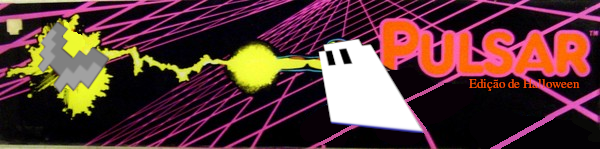
\includegraphics[scale=1.3]{banner}
\caption{Banner do jogo Pulsar editado para a nossa versão do jogo}
\end{figure}

\section{Metodologia}

\subsection{Música e efeitos sonoros}

O jogo possui três músicas, uma de início, quando o jogador inicia o jogo; outra de derrota, quando o jogador morre no jogo; e uma de vitória, quando o jogador vence o jogo.

Cada uma dessas teve que ser manualmente composta usando as ferramentas disponibilizadas no RARS. A partir de syscalls, sons podem ser reproduzidos e dessa forma uma música pode ser simulada, com acordes, ritmo e harmonia.

As músicas em si são todas compostas de sons e músicas culturalmente famosas. A música de derrota é uma derivação do efeito sonoro de suspense famoso "Dun dun duuun!" (comumente nomeado assim\textsuperscript{\cite{b3}})
logo a música de vitória é o conjunto dos sete primeiros acordes após a introdução de Marche Funèbre\textsuperscript{\cite{b4}}

\begin{figure}[h]
\centering
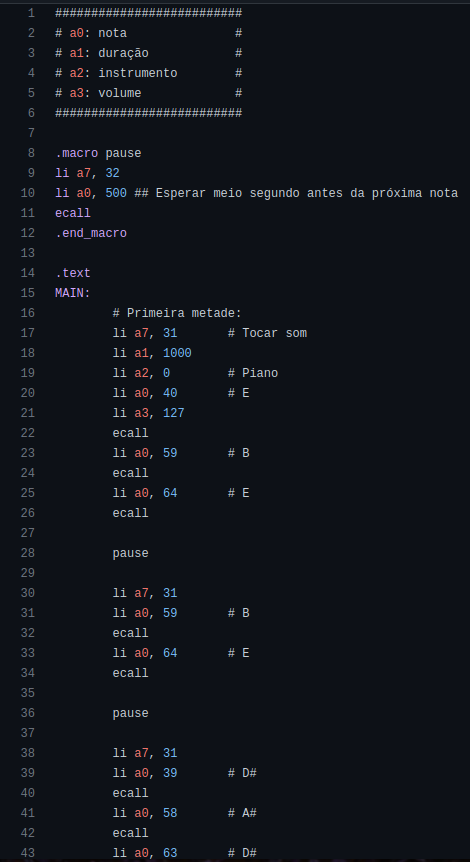
\includegraphics[scale=0.3]{codigo_de_musica}
\caption{Exemplo de um dos códigos de música para o jogo}
\end{figure}  

Usamos de auxílio tutoriais de piano disponibilizados no YouTube para que pudéssemos saber as notas e suas durações de cada música.

Quanto aos efeitos sonoros foi preciso apenas usar o syscall 31 do RARS, onde no registrador a2 é guardado um valor intermediário específico entre 120 à 127. Pois estes são os valores dedicados aos próprios efeitos sonoros que o RARS possui.

\subsection{Arte visual}
Seguindo a temática de Halloween, decidimos utilizar uma paleta de cores de tons escuros para denotar o aspecto misterioso e assustador proporcionado pela data comemorativa. Ela foi utilizada na elaboração do mapa da casa assombrada que o jogador deverá escapar. A tela inicial do jogo, por exemplo, é composta por vários tons de marrom para simbolizar o material em que a casa foi construída, no caso madeira, além de trazer a ideia de um local escuro e abandonado.
\begin{figure}[H]
\centering
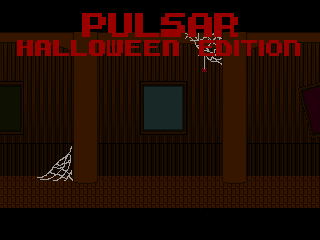
\includegraphics[scale=0.7]{tela_inicio}
\caption{Tela inicial que recebe o jogador}
\end{figure}  

Os desenhos dos inimigos foram inspirados por animais comumente encontrados em locais escuros e que as pessoas têm medo. Tendo isso em vista, escolhemos o rato e morcego para implementarmos no jogo.
O personagem controlado pelo jogador é baseado na clássica cartoonização de um fantasma, um pano branco com dois olhos pretos.

\begin{figure}[h]
\centering

\includegraphics[scale=0.7]{fantasma}
\caption{Sprite do fantasma}
\end{figure}  

Sabendo que a utilização de cheats na apresentação foi aconselhada, desenhamos um novo desing para o jogador que, ao estar sob efeito do cheat, mudaria a cor de seu pano branco para um azul escuro, fazendo assim uma referência ao modo de como os fantasmas do jogo arcade japonês "Pac-Man" (1980)\textsuperscript{\cite{b6}} ficavam quando o jogador coletava uma "power pellets" no video-game.
\begin{figure}[h]
\centering

\includegraphics[scale=0.7]{fantasma_cheat}

\includegraphics[scale=0.7]{fantasma_pacman}
\caption{Sprite do fantasma}
\end{figure}  

Para os tiros, pensamos do fantasma atirar ectoplasma como seu ataque contra os inimigos do mapa. O personagem "Geleia" do filme "Os Caça-Fantasmas" de 1984 foi grande parte da inspiração do desing do projétil.

\begin{figure}[H]
\centering

\includegraphics[scale=0.3]{ectoplasma_modelo}
\caption{Sprite do ataque do jogador}
\end{figure}  

Em prol de manter a natureza de um jogo arcade, utilizamos a fonte do jogo "Super Mario World" (1990) na cor vermelha como a fonte do nosso projeto, realizando suas devidas adaptações tais como a criação de letras maiúsculas e minúsculas visto que não havia diferença no jogo original. 

\begin{figure}[H]
\centering
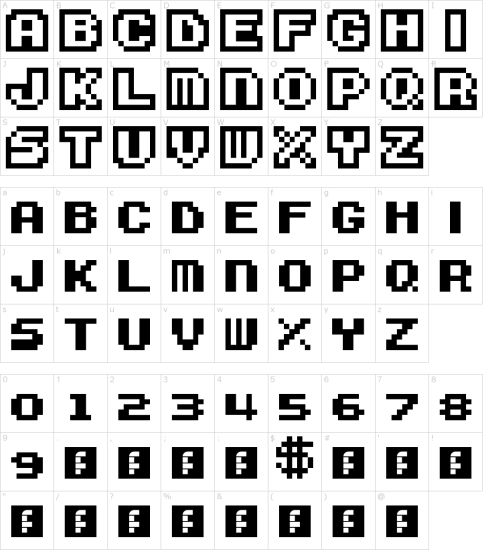
\includegraphics[scale=0.3]{fonte}
\caption{Fonte do jogo}
\end{figure} 

Utilizamos como molde para o mapa do jogo em si o mapa em formato de labirinto presente em "Pulsar". Entretanto, o adaptamos para que a ideia de casa abandonada esteja presente em toda jogabilidade.

\begin{figure}[H]
\centering
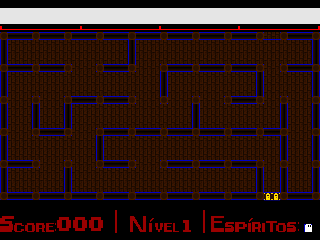
\includegraphics[scale=0.9]{mapa_fase_1}
\caption{Modelo do mapa da primeira fase do jogo}
\end{figure}  

\subsection{Lógica do jogo}

A base utilizada para o desenvolvimento das mecânica que foram utilizadas no jogo foi a estrutura do diagrama (Fig. 6) que criamos para facilitar a direção do desenvolvimento.

\begin{figure}[h]
\centering
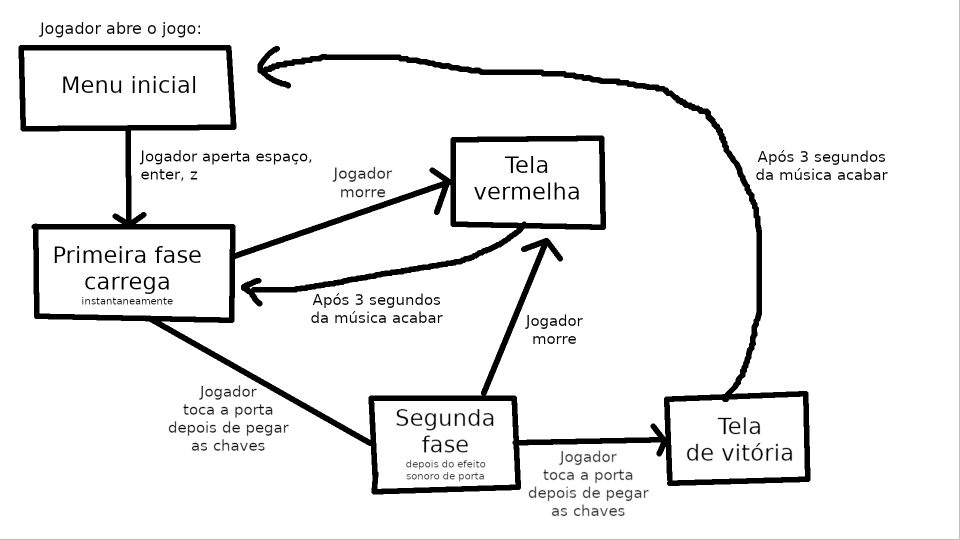
\includegraphics[scale=0.2]{diagrama}
\caption{Diagrama da estrutura do nosso jogo}
\end{figure}

Por meio do diagrama, foi possível desenvolver a estrutura básica para a troca entre as diferentes etapas do jogo, que são: Tela de Início, Fase 1, Fase 2, Tela de Morte e Tela de Vitória.

Outra mecânica importante definida a partir do diagrama foram as condições que levariam para as mudanças entre as diferentes etapas, o que guiou o desenvolvimento do trabalho.

Para o desenvolvimento das mecânicas internas do jogo, as quais não foram claramente definidas no diagrama base, foram desenvolvidos diferentes métodos para atingir os objetivos desejados. As mecânicas, com seus respectivos métodos, foram exemplificadas nos próximos tópicos.

\subsubsection{Sistema de colisão}
 O sistema de colisões e coletas de chaves foram baseados na análise das cores dos pixeis nos arredores dos personagnes, tiros e inimigos. Comparando as diferentes cores possíveis tornou-se possível determinar as reações esperadas para cada um dos casos e tornava um único código capaz de atender todos os objetivos citados.

\begin{figure}[h]
\centering

\includegraphics[scale=0.7]{sistema_de_colisao}
\caption{Representação do sistema de colisão entre o personagem e as paredes do jogo}
\end{figure}  

Tendo a figura 7 como exemplo do funcionamento desse código, podemos observar que a parede possui uma cor específica em sua volta que foi definida como o código hexadecimal 0xC7, a qual é interpretada pelo Rars como inivisível. Fazendo uso dessa cor apenas para as paredes e o personagem tornou-se possível detectar quando teria uma colisão com objetos que não possuiam reação.

Além disso, o mesmo método foi usado para determinar a colisão de tiros com inimigos, coleta de chaves, passagem de fase e danos causados por inimigos, cada um fazendo uso de uma cor distinta para facilitar a interpretação e evitar possíveis ambiguidades no código.
\subsubsection{Movimentação do personagem} 
  A movimentação do personagem, dos inimigos e dos tiros e a limpeza de rastros foram baseados em labels que continham  os valores da posição anterior e atual dos alvos da análise. As labels contém os valores X e Y de cada objeto que se move no jogo, os quais podem ser acessados por outras partes do código, possibilitando o uso dessas informações não só para a movimentação do personagem como também para a limpeza de rastros e o funcionamento do sistema de colisões.
  
\subsubsection{Inteligência dos inimigos} 
A inteligência dos inimigos criados para o jogo foi baseada no sistema de colisão, no sistema de movimentação do personagem e no sistema de tiros. Por meio da junção desses sistemas foi possível criar uma imagem que se move em uma direção determinada e troca seu curso baseado nas colisões que sofre.

\begin{figure}[h]
\centering
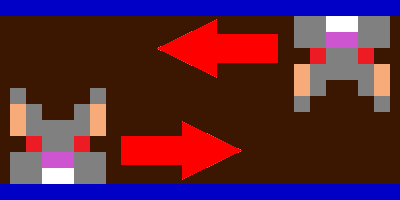
\includegraphics[scale=0.7]{rato_movimento}
\caption{Ilustração de movimento do inimigo rato}
\end{figure}  

o movimento dos ratos é em um único eixo, podendo ser para direita ou para esquerda. Esse mesmo conceito foi utilizado para os demais inimigos empregados no jogo.
 
\subsubsection{Sistema de chaves}  
O sistema de chaves e portas foi feito com o uso de...

\begin{figure}[H]
\centering

\includegraphics[scale=1]{chave_e_porta}
\caption{Imagem com a chave e sua respectiva porta}
\end{figure}

O Sistema de score foi feito... 

[Imagem com o Score]

\section{Resultados Obtidos}
No geral, nossas dificuldades foram superadas e conseguimos criar um jogo completo, com início, meio e fim. 

O tema que tinhamos em mente foi implementado com sucesso assim como as técnicas que elaboramos para a execução do projeto. 

Como resultado, a equipe adquiriu um melhor entendimento das mecânicas para o desenvolvimento em Assembly e a lógica de programação em Assembly na arquitetura RISC-V, assim como noções de desenvolvimento em baixo nível, como gestão manual de memória e planejamento de um projeto com recursos limitados.

Apesar de não termos conseguido implementar uma música de fundo para tocar durante o jogo, nós conseguimos implementar várias músicas, cada uma para situações diferentes no jogo, melhorando a experiência de jogador.

Em relação a arte visual do jogo, esta foi bem executada, conseguimos criar um sprite\textsuperscript{\cite{b5}} para todos os objetos e personagens do jogo 

Alguns dos detalhes que tinhamos como planejamento não foram implementados, porém a falta desses detalhes não atrapalha de nenhuma maneira a experiência do jogador.

\section*{Conclusão}

Tendo em vista os pontos observados

\begin{thebibliography}{00}
\bibitem{b1} \url{https://www.arcade-museum.com/game_detail.php?game_id=9150} 

\bibitem{b2} \url{https://riscv.org/about/}

\bibitem{b3} \url{https://en.wikipedia.org/wiki/Dun_dun_duuun!\#CITEREFSuspense1942}

\bibitem{b4} \url{https://youtu.be/hZY5DBmgC_A}

\bibitem{b5} \url{https://pt.wikipedia.org/wiki/Sprite_(computa%C3%A7%C3%A3o_gr%C3%A1fica)}

\bibitem{b6} \url{https://pt.wikipedia.org/wiki/Pac-Man}

\end{thebibliography}
\vspace{12pt}

\end{document}
